\hypersetup{
  pdftitle={A Formal Specification of the Cardano Ledger},
  breaklinks=true,
  bookmarks=true,
  colorlinks=false,
  linkcolor={blue},
  citecolor={blue},
  urlcolor={blue},
  linkbordercolor={white},
  citebordercolor={white},
  urlbordercolor={white}
}


  \cleardoublepage%
  \tableofcontents%
  \listoffigures%
  \clearpage%

  \begin{changelog}
        \change{2019/10/08}{Jared Corduan, Polina Vinogradova and Matthias G\"udemann}{FM (IOHK)}{Initial version (0.1).}
        \change{2019/10/08}{Kevin Hammond}{FM (IOHK)}{Added cover page.}
      \end{changelog}
      \clearpage%
\begin{landscape}
\floatstyle{plain}
\restylefloat{figure}
\begin{figure*}
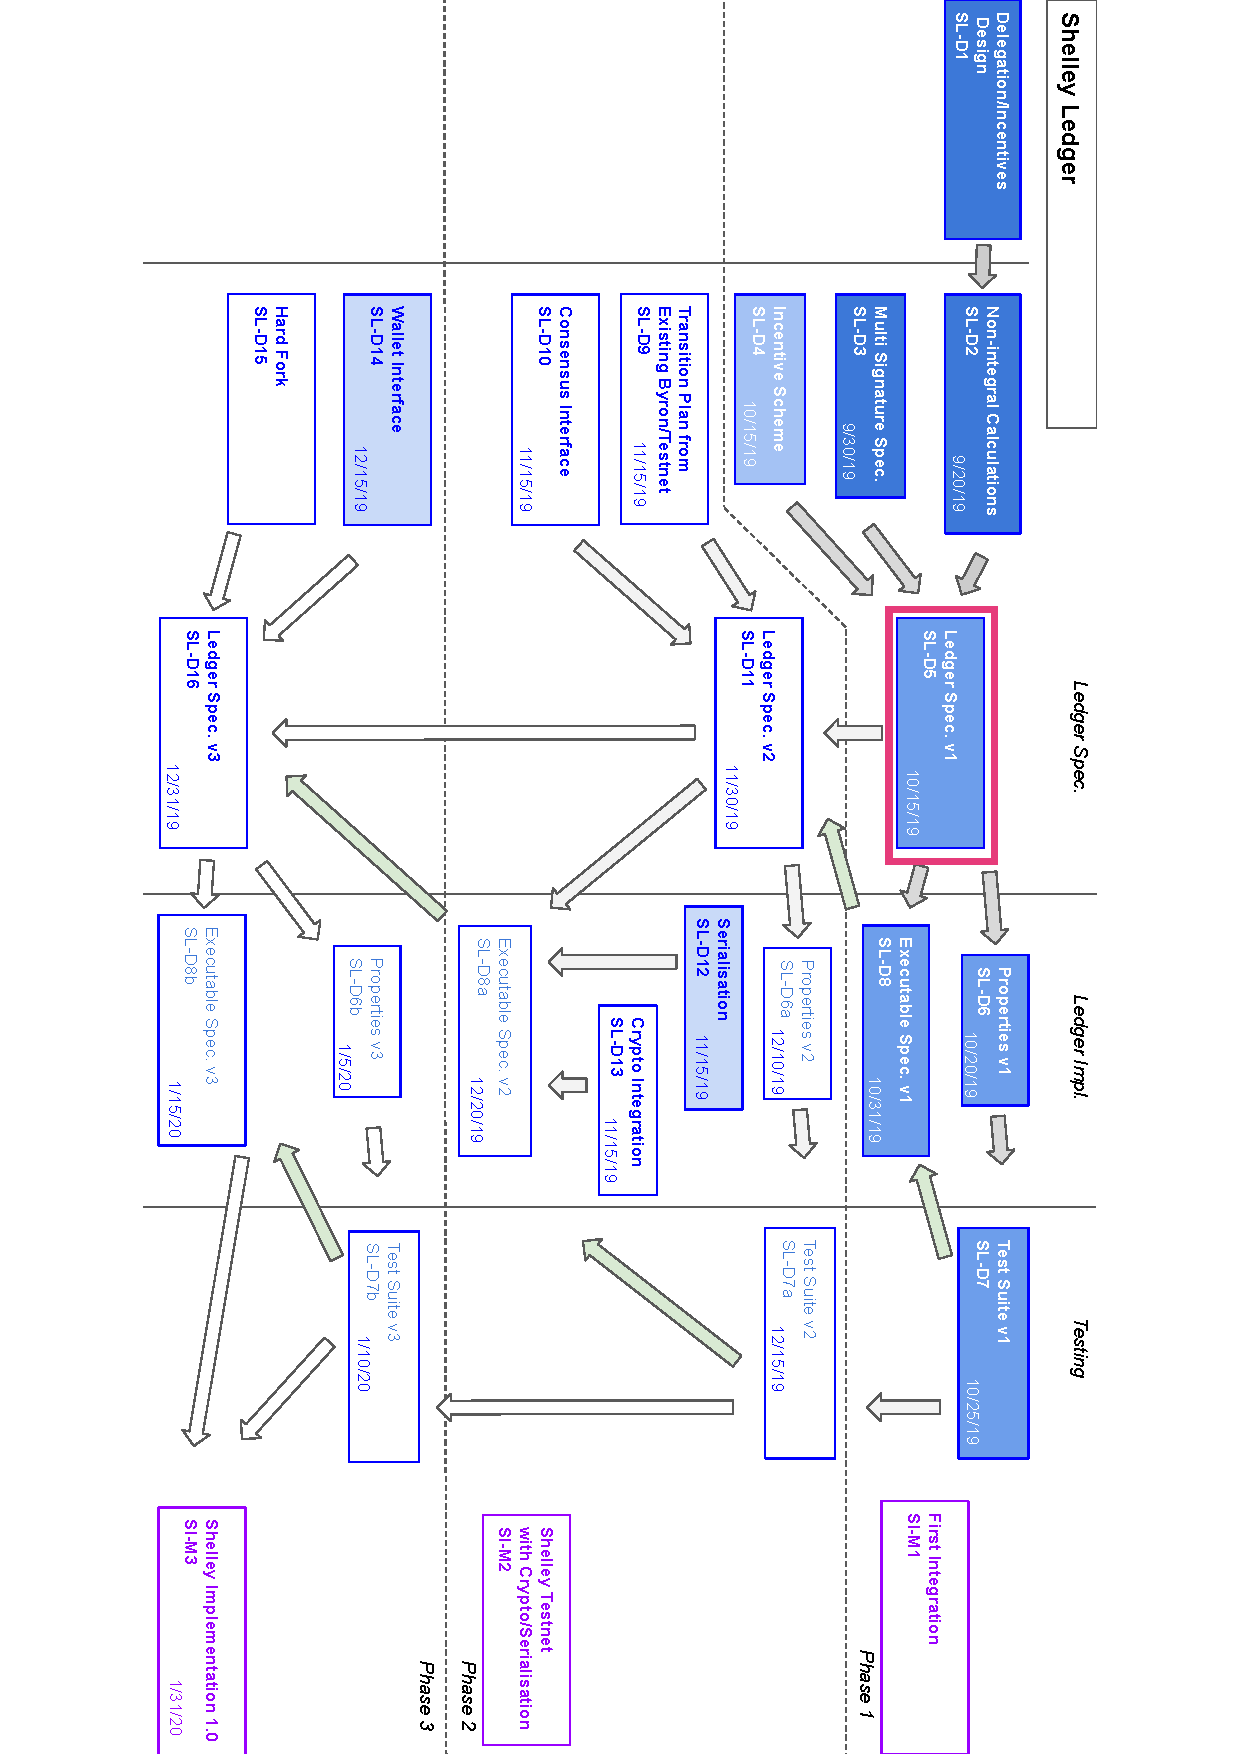
\includegraphics[scale=0.8,angle=90]{d5-depends.pdf}
\caption{Positioning of this Deliverable (outlined in red).}
\end{figure*}
\end{landscape}
\floatstyle{boxed}
\restylefloat{figure}
\cleardoublepage
\renewcommand{\thepage}{\arabic{page}}
\setcounter{page}{1}

\title{A Formal Specification of the Cardano Ledger}

\author{Jared Corduan  \\ {\small \texttt{jared.corduan@iohk.io}} \\
   \and Polina Vinogradova \\ {\small \texttt{polina.vinogradova@iohk.io}} \\
   \and Matthias G\"udemann  \\ {\small \texttt{matthias.gudemann@iohk.io}}}

%\date{}

\maketitle

\begin{abstract}
This document provides a formal specification of the Cardano ledger for use in the upcoming Shelley implementation.
It is intended to underpin a Haskell executable specification that will be the basis of the initial
Shelley release, and represents a core design and quality assurance document.
It will be used to define properties and tests, and to provide the basis for strong formal assurance
using mathematical proof techniques.
The document defines the rules for extending the ledger with transactions
that will affect both UTxO and stake delegation.
Key properties that have been identified include the preservation of balances, absence of double spend, stakepool registration,
and reward splitting.
\end{abstract}

\section*{List of Contributors}
\label{acknowledgements}

Nicol\'as Arqueros,
Nicholas Clarke,
Duncan Coutts,
Ruslan Dudin,
Sebastien Guillemot,
Kevin Hammond,
Vincent Hanquez,
Ru Horlick,
Michael Hueschen,
Yun Lu,
Philipp Kant,
Jean-Christophe Mincke,
Damian Nadales,
Nicolas Di Prima.
